\section{Conclusion}
\label{section:conclusion}

% TODO bigger grid

A promising modified XCS approach has been investigated to overcome the drawbacks of the standard XCS algorithm concerning NOMDPs. The proposed idea is mainly based on expanding the local reward function and adding some kind of temporary memory, which stores past action sets and their corresponding reward values. Local payoffs can be delayed and analyzed later. Thus, the reward function reflects better the local agent's behavior. The experiments have shown that this new approach is superior to the standard XCS algorithm, mainly due to its ability to work well with advanced local reward functions -- an ability which XCS seemingly lacks. Besides improving the new algorithm itself, future work will focus on an intelligent switching strategy between \emph{explore} (when no prey is in sight) and \emph{exploit phases} (when a predator is near by the prey). In addition, improvement is expected by an adaptive \emph{learning rate} $\beta$ and an adaptive \verb|maxStackSize| to fit the current scenario's needs. Finally, it seems interesting to test the \emph{eventXCS} approach on larger grids and on standard Maze scenarios or other NOMDPs from literature.

% Cooperation (incorporated in the reward function) is more or less achieved through rejection and attraction. Predators reject each other, the prey attracts the predators. Thus, agents try to uniformly distribute on the grid and observation time of the prey seems to be maximized. In addition it is shown that the new XCS approach retains its ability to recognize local obstacle configurations in order to reach the goal object.
%In Section~\ref{section:experimental-results} it was shown that SXCS outperforms XCS in scenarios with few obstacles. This was mainly due to the fact that XCS is unable to handle base reward functions that differ from the global goal and because XCS seems to have problems reaching a stable level, possibly due to overlearning. 
%SXCS with \emph{best selection} showed serious problems in the \emph{difficult scenario} while it was able manage the problem with a more random \emph{tournament selection}. This points to a correctable flaw in the design of the algorithm (probably with the \emph{neutral events}). But other than XCS SXCS \emph{can} handle advanced base reward functions, e.g. with a collaborative element (evading other agents) which significantly helps for example in the \emph{difficult scenario} though this is probably due to the fact that it simply encourages agents to move away from other agents, explore the grid and move through the openings. But in the end SXCS was designed to follow and observe a moving prey, the \emph{difficult scenario} is more like a labyrinth where finding the prey in the first place is important.

% \begin{itemize}

% \item A good local evaluation function for the XCS can be constructed on the base of a heuristic with good performance (see Section~\ref{subsection:environment_reward_function}).

% TODO!
% \item By adding external memory that records the reward history (see Section~\ref{subsection:reward_distribution}) the newly created algorithm SXCS can solve the problem much better than XCS (see Section~\ref{section:experiments}).

% \item A variation of the learning rate $\beta$ can be successful depending on the scenario (see Section~\ref{subsection:learning_rate} and Section~\ref{subsection:xcs_difficult_scenario} for the difficult scenario respectively).

% \item Die Agenten mit XCS und SXCS haben deutliche Probleme mit Szenarien mit vielen Hindernissen (siehe Kapitel~\ref{subsection:tournament_factor_test}). TODO

% \item Ein dynamischer Wechsel der Auswahlart f�r Aktionen w�hrend eines Laufs kann sinnvoll sein, um die Zahl der blockierten Bewegungen zu verringern und das Zielobjekt besser verfolgen zu k�nnen (siehe Kapitel~\ref{subsection:analysis_random_scenario_xcs}). TODO

% \item XCS as well as SXCS can solve difficult scenarios with positions of interest significantly better than randomly moving agents. Under certain circumstances SXCS can solve this scenario even better than the heuristic on which its evaluation function is based on (see Section~\ref{subsection:xcs_difficult_scenario}).

% \end{itemize}

% binary function
% This causes some problems when trying to model the heuristic as it is impossible to distinguish situation with e.g. one other agent and four other agent in sight. Probably a better implementation would be to count the number of agents and return it as a reward. An additional problem surfaces in scenarios with a relatively low number of agents because the reward function returns 1 most of the time. This could harm the learning process.

% \begin{figure}[ht]
% \centerline{	
% 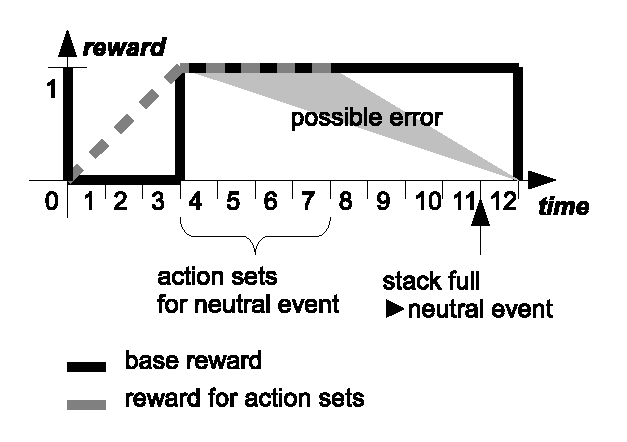
\includegraphics[scale=0.75]{neutral_reward}
% }
% \caption{Schematic display of the reward distribution to the action sets after a neutral event (with \emph{base reward} = 1)}
% \label{figure:neutral_reward}
% \end{figure}

% In XCS wird lediglich die jeweils letzte \emph{action set} Liste aus dem vorherigen Schritt gespeichert. In der neuen Implementierung werden dagegen eine ganze Anzahl (bis zum Wert \emph{maxStackSize}) von \emph{action set} Listen gespeichert. Die Speicherung erlaubt zum einen eine Vorverarbeitung des \emph{reward} Werts anhand der vergangenen Schritte und auf Basis einer gr��eren Zahl von \emph{action set} Listen und zum anderen die zeitliche Relativierung einer \emph{action set} Liste zu einem Ereignis. Die \emph{classifier} werden dann jeweils r�ckwirkend anhand des jeweiligen \emph{reward} Werts aktualisiert, sobald bestimmte Bedingungen eingetreten sind.

% Bei der Benutzung eines solchen Stacks entsteht eine Zeitverz�gerung, d.h. die \emph{classifier} erhalten jeweils Informationen, die bis zu \emph{maxStackSize} Schritten zu alt sein k�nnen. Tritt beim Stack ein �berlauf auf, gab es also \emph{maxStackSize} Schritte lang keine �nderung des \emph{base reward} Werts mehr, dann wird abgebrochen und die \(\frac{maxStackSize}{2}\) �ltesten Eintr�ge werden vom Stack genommen. Alle diese Eintr�ge werden dabei vorher mit einem \emph{reward} Wert aktualisiert, der diesem \emph{base reward} Wert entspricht.

% In such a case 

% There are two drawbacks with this implementation: Firstly there is a time delay of the reward distribution because it is impossible to foresee when an event will occur. Secondly, in the case of a neutral event, the prediction of future events could be wrong and a new positive or negative event occurs shortly after the neutral event (see Figure~\ref{figure:neutral_reward}). Both points do not seem significant because the time delay, compared to the standard implementation with repetition of the problem, is very small and the erroneous reward distribution in the case of a neutral event could be corrected retroactively to a certain degree. On the other hand recording the history of rewards could provide a basis for a deeper analysis resulting in a better reward distribution than the one that is presented here.

% \subsection{Implementation of SXCS}

% The original implementation~\cite{But00} of XCS allows a modular setup of the environment so that the reward function (see Section~\ref{subsection:reward_function}) can be calculated in the environment module. As explained in Section~\ref{subsection:reward_distribution} and ~\ref{subsection:events} additional recording and analysis of the base reward generated by the reward function is necessary. Thus some parts of the code need to be rewritten resulting in the following modified version of the code:
% TODO Code?

